 \documentclass[a4paper]{amsart}

\usepackage{color}
\usepackage[colorlinks=true, citecolor=red]{hyperref}  %needs to come before amsrefs package to work with \cite{}*{}
\usepackage{amssymb,latexsym}
\usepackage[alphabetic]{amsrefs}
\usepackage[mathscr]{eucal}
\usepackage{pdfsync}
\usepackage{graphicx}
\usepackage{epstopdf}
\DeclareGraphicsRule{.tif}{png}{.png}{`convert #1 `dirname #1`/`basename #1 .tif`.png}
\usepackage[all]{xy}
\usepackage{titletoc}
%\usepackage{showkeys}  %options notref  notcite 

\input{rgb.tex}

\CompileMatrices

\theoremstyle{plain}
\newtheorem{theorem}{Theorem}[section]
\newtheorem{lemma}[theorem]{Lemma}
\newtheorem{proposition}[theorem]{Proposition}
\newtheorem{corollary}[theorem]{Corollary}

\theoremstyle{definition}
\newtheorem{definition}[theorem]{Definition}%[section]


\theoremstyle{remark}
\newtheorem{defn}[theorem]{Definition} 
\newtheorem{example}[theorem]{Example}
\newtheorem{remark}[theorem]{Remark}
\newtheorem{discussion}[theorem]{Discussion}

%\numberwithin{equation}{section}

%\newcommand{\abs}[1]{\lvert#1\rvert}

\DeclareMathOperator{\Lip}{Lip}
\DeclareMathOperator{\dist}{dist}
\DeclareMathOperator{\expected}{\mathbb{E}}
\DeclareMathOperator{\prb}{Prob}
\DeclareMathOperator{\spt}{spt}
\DeclareMathOperator{\lap}{\Delta}
\DeclareMathOperator{\Tr}{Tr}

\raggedbottom

\addtolength{\textwidth}{2cm}
\addtolength{\oddsidemargin}{-1cm}
\addtolength{\evensidemargin}{-1cm} 
\addtolength{\topmargin}{-1cm} 
\addtolength{\textheight}{2cm}

\setcounter{tocdepth}{3}



%%% BEGIN DOCUMENT
\begin{document}

\title{Notes and Remarks}  
\author{John E.\ Hutchinson}
\date{\today}

%\begin{abstract} 
%\end{abstract}

\maketitle

\tableofcontents


%%%%%%%%%%%%%%%%%%%%%%%%%%%%%%%%
%%%%%%%%%%%%%%%%%%%%%%%%%%%%%%%%
%%%%%%%%%%%%%%%%%%%%%%%%%%%%%%%%
%%%%%%%%%%%%%%%%%%%%%%%%%%%%%%%%
\section{\textbf{13/5/09: Generation Process for $ V $-Variable Fractals}} 

In the following we see how one run of the backward process for generating $ V $-variable fractals can be interpreted as \emph{cell division to grow a  \underline{single}  \emph{($ V $-variable)} organism}.

On the other hand, we see how one run of the forward process for generating $ V $-variable fractals can be interpreted as  \emph{interbreeding organisms to produce  arbitrarily large  \underline{families}
of  \emph{($ V $-variable)} organisms} whose empirical distributions approximate  the natural distribution on $ V $-variable fractals.

One run of either  process  is governed by an infinite sequence of $ V $-tuples of transformation rules.  For the backward process the transformations are interpreted as \emph{cell replacement} rules.   For the forward process  the transformations are interpreted  as \emph{organism combination} rules.  The results are related, but also very different.


%%%%%%%%%%%%%%%%%%%%%%%%%%%%%%%%%%%%%%%%%
%%%%%%%%%%%%%%%%%%%%%%%%%%%%%%%%%%%%%%%%%
\subsection{Backward Process as   Cell Division}  

\begin{figure}[htbp] %  figure placement: here, top, bottom, or page
   \centering
   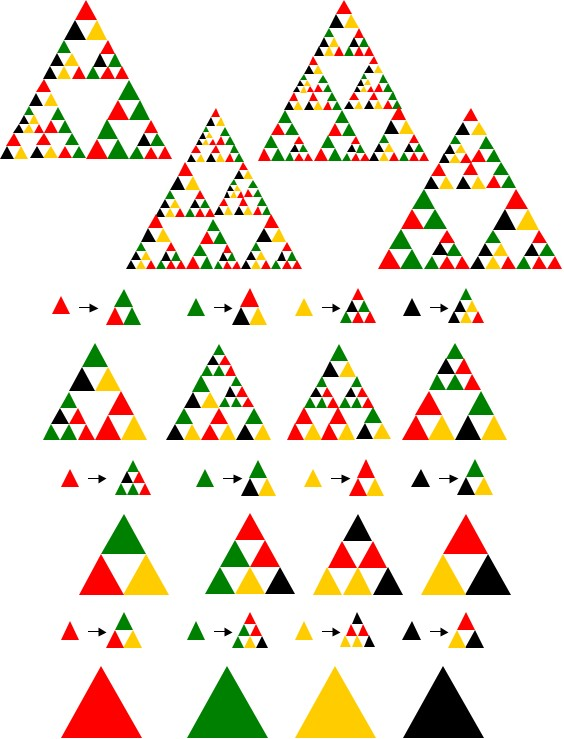
\includegraphics[width=5in]{V-vargenA.jpg} 
   \caption{\small \textbf{Backward Process.} The transformations rules are interpreted as \emph{replacement/division}   rules. \newline
 \mbox{} \quad  The bottom line shows the four possible types for the initial cell.  The   division rules at time 1 are shown next and  are followed by the 4 resulting organisms at time 1.  The transformation rules at time 2 are then followed by the resulting organisms at time 2.  Finally, the transformation rules at time 3 are followed by the resulting organisms at time 3. 
  \newline  \mbox{}  \quad  Now observe any of the four  growing organisms at successive times and ignore the cell type, i.e.\ colour. 
 The organism structure at each time is a refinement  of the organism at the previous time.  This is more easily seen in Figure~\ref{V-vargenblack}, where colours are suppressed and the development beginning from the green cell is shown.}
   \label{V-vargenA}
\end{figure}

\begin{figure}[htbp] %  figure placement: here, top, bottom, or page
   \centering
   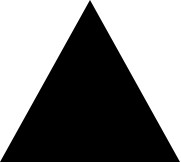
\includegraphics[width=1in]{V-vargenblack0.jpg} \quad 
   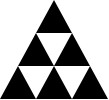
\includegraphics[width=1in]{V-vargenblack1.jpg} \quad 
   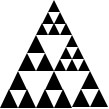
\includegraphics[width=1in]{V-vargenblack2.jpg} \quad 
   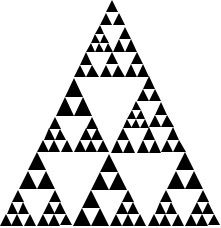
\includegraphics[width=1in]{V-vargenblack3.jpg} 
   \caption{\small Organism development via cell division.  Note how each embryo is a refinement of the embryo at the previous time.}
   \label{V-vargenblack}
\end{figure}




\emph{See Figure~\ref{V-vargenA} where $ V=4 $.}

Each cell  is  one of $ V $ possible types,  where the integer $ V $ is fixed.  Here we take $ V=4 $ and types are
indicated by the colours red, green, yellow and black.
Organism growth is determined by an infinite sequence of $ V $-tuples of transformations, here interpreted as  \emph{replacement} or \emph{cell division} rules.  

Begin with the initial cell at time $ t=0 $. At  times $ t = 1,2,3,\dots $,  cell division   occurs according to a $ V $-tuple of  replacement rules as indicated in Figure~\ref{V-vargenA}.
The kind of cell division, or equivalently the replacement rule applied to a cell, depends on the type of the cell, but the $ V$-tuple of transformation rules depends on the external environment at the time of  division.



\medskip
If we \emph{disregard} the information regarding  individual cell type, we see the sequence of embryos at each division time converges to a limit adult organism (fractal).   Cell type/colours are a book-keeping device and not part of the structure of the limit organism/fractal. See Figure~\ref{V-vargenblack} where the initial cell was of ``green'' type.



%%%%%%%%%%%%%%%%%%%%%%%%%%%%%%%%%%%%%%%
\subsection{Forward Process as Organisms Breeding} \label{fpob}


\begin{figure}[htbp] %  figure placement: here, top, bottom, or page
   \centering
   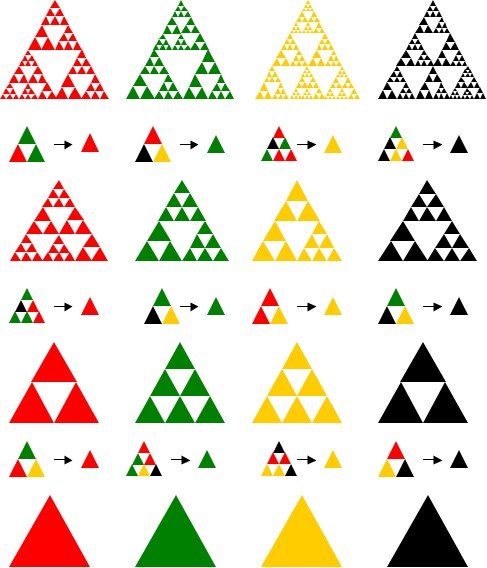
\includegraphics[width=5in]{V-vargenB.jpg} 
   \caption{\small \textbf{Forward Process.} The transformations rules are interpreted as \emph{combination}   rules. \newline
 \mbox{} \quad  
 Begin with one individual organism of each type, ignoring any fine detail.  The first set of combination rules produce 4 new organisms, one  of each type.  The second set produces another 4 and the third set produces another 4.  After a few initial iterations, successive iterations produce a collection of organisms, 4 for each iteration, whose empirical distribution converges to the theoretical distribution of $ V $-variable fractals.}
   \label{V-vargenB}
\end{figure}


Here we work with entire organisms rather than individual cells.
Types now refer to organisms and can again be regarded as a bookkeeping device.
Each individual organism  will be  one of $ V $ possible types.   
See Figure~\ref{V-vargenB} where $ V=4 $ and the type of an individual organism  is indicated by the colours red, green, yellow and black.
An entire \emph{infinite family} of organisms  is now generated by a single infinite sequence of $ V $-tuples of transformations, where the transformations are now interpreted as  \emph{combination} or \emph{reproduction} rules.  

Begin with $V $ individual organisms  at time $ t=0 $, one for each type. At  times $ t = 1,2,3,\dots $,  breeding   occurs according to a $ V $-tuple of  combination rules as indicated in Figure~\ref{V-vargenA}.
At each generation there is one new organism produced for   each type, as determined by the  relevant transformation rule, 
and the $ V$-tuple of transformation rules again depends on the external environment at the time of  breeding.

We have used the same sequence of rules in Figure~\ref{V-vargenB} as in Figure~\ref{V-vargenA}.  

%%%%%%%%%%%%%%%%%%%%%%%%%%%%%%%%%
\subsection{The Forward, Backward and Retarded Processes}   *** Incomplete***   The \emph{forward process} for $ SG(2) $ consists of selecting a starting point $ x_0 $ and a sequence of maps $ (g_i)_{i\geq 1} $ from $ F=\{ f_1,f_2,f_3  \} $ in an iid manner according to some fixed probability distribution $ P $.  Then the sequence of points
\[
x_0,\  x_1=g_1(x_0),\  x_2 = g_2\circ g_1(x_0), \  g_3\circ g_2 \circ g_0 (x_0),                   \dots ,
\]
converges a.s.\  to $  SG(2) $.       
More precisely, the sequence of unit measures
\[
\frac{1}{n} \big(\delta_{x_0}+\cdots + \delta_{x_{n-1}}\big)
\]
converges in the weak sense of measures to the natural measure on $ SG(2) $ induced from $ P $.

The \emph{backward process} says that for any initial non empty compact $ K $, the sequence of sets
\[
K, F(K), F^{\circ 2}(K), F^{\circ 3}(K), \dots \to SG(2),\]
in the Hausdorff  sense, where 
\[ F(E) := f_1(E) \cup f_2(E) \cup f_3(E). \]

The \emph{retarded} process takes sequences of the form:
\[
x_0,  \  x_1 = g_1(x_0),\  x_2 = g_1\circ g_2(x_0),\  x_3 = g_1\circ g_2 \circ g_3 (x_0), \dots 
\]
Note the order of composition.  Each sequence will converge to a point on $ SG(2) $.  Running the process many times gives a sample of points on $ SG(2) $ whose empirical distribution converges a.s.\ to the natural distribution on $ SG(2) $ given by $ P $.


\bigskip
\emph{The previously described forward process for $ V $-variable fractals is the forward process on the superfractal attractor.   The backward process is really  the retarded process on the superfractal attractor.}



%%%%%%%%%%%%%%%%%%%%%%%%%%%%%%%%%
\subsection{DNA}   *** Incomplete*** A possible model for DNA reproduction is a variation of Section~\ref{fpob} as follows.   ***The idea is to think of the organisms as a pair of DNA molecules.  The allowable combinations correspond to crossing over.  This needs to be formalised***    






%%%%%%%%%%%%%%%%%%%%%%%%%%%%%%%%%
\subsection{The Class of $ V $-Variable Fractals}
In the backward process we saw how a single organism (or fractal) was generated from an initial cell by a sequence of $ V $-tuples of  transformations  chosen for example from a given collection $\mathfrak{F}$ of $ V $-tuples of transformations.  The collection of all possible $ V $-variable fractals obtained in this manner is denoted by $ \mathcal{K}_V $
and is called \emph{the set of $ V$-variable fractals}. Clearly,
\[
\mathcal{K}_1 \subset \mathcal{K}_2 \subset \cdots .
\] 
The collection $ \mathcal{K}_1 $ is  the collection of homogeneous fractals in the sense of Hambly.  Moreover, $ \mathcal{K}_V \uparrow    \mathcal{K}_\infty$ as $ V\to \infty $, where $    \mathcal{F}_\infty $ is the collection of recursive fractals in the sense of Falconer, Graf, and  Mauldin and Williams. 

%%%%%%%%%%%%%%%%%%%%%%%%%%%%%%%%%%
\subsection{Contractive Maps  and IFSs}  
Each of the 4 transformation rules in Figures~\ref{V-vargenA} and~\ref{V-vargenB} corresponds to an IFS for the Sierpinski gasket $ SG(2) $ or $ SG(3) $,  if one disregards the colour information corresponding to the cell type or organism type.
However, there is a convenient way to also incorporate this information.  

Each 4-tuple of transformation rules    corresponds to a map
\begin{equation} \label{4t} 
 \boldsymbol{\Phi} : \Big(\mathcal{K}(\mathbb{R}^2 ) \Big)^4    \to \Big(\mathcal{K}(\mathbb{R}^2 ) \Big)^4,\quad 
 \boldsymbol{\Phi}(K_1,\dots, K_4)  = \Big(\Phi_1(K_1,\dots, K_4), \dots, \Phi_4(K_1,\dots, K_4)\Big),
\end{equation} 
where  $ \mathcal{K}(\mathbb{R}^2)$ is the set of non empty compact subsets of $ \mathbb{R}^2 $.
More precisely, identify  the colours red, green, yellow and black respectively with the four coordinates in the natural order in~\eqref{4t}. Let the IFSs  for $ SG(2) $ and $ SG(3) $ be $ F=(f_1,f_2,f_3) $  and $ (G=(g_1,\dots, g_6) $ respectively with notation as shown in Figure~\ref{SG}. 
\begin{figure}[htbp] %  figure placement: here, top, bottom, or page
   \centering
   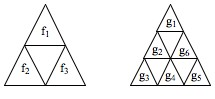
\includegraphics[width=2in]{SGmaps.jpg} 
   \caption{\small The IFS $ F=(f_1,f_2,f_3) $ for $ SG(2) $ and $ G=(g_1,\dots, g_6)$ for $ SG(3) $.}
   \label{SG}
\end{figure}

Then the map $  \boldsymbol{\Phi}^3 =   (\Phi^3_1, \Phi^3_2, \Phi^3_3, \Phi^3_4 )$, corresponding to the third 4-tuple of transformations in Figures~\ref{V-vargenA} and~\ref{V-vargenB},  is given by
\begin{align*}
\Phi^3_1(K_1,K_2,K_3,K_4) &= f_1(K_2)\cup f_2(K_1) \cup f_3(K_2), \\
\Phi^3_2(K_1,K_2,K_3,K_4) &= f_1(K_1)\cup f_2(K_4) \cup f_3(K_3), \\
\Phi^3_3(K_1,K_2,K_3,K_4) &=g_1(K_1)\cup g_2(K_4) \cup g_3(K_2)\cup g_4(K_1)\cup g_5(K_1) \cup g_6(K_2), \\
\Phi^3_4(K_1,K_2,K_3,K_4) &= g_1(K_2)\cup g_2(K_4) \cup g_3(K_4)\cup g_4(K_3)\cup g_5(K_1) \cup g_6(K_3).
\end{align*} 
The maps $  \boldsymbol{\Phi}^1 $ and $  \boldsymbol{\Phi}^2 $ corresponding to the first and second rows of transformations are defined similarly.

Let $ \boldsymbol{A} = (A_1,A_2,A_3,A_4) $ denote the first 4-tuple of sets in Figures~\ref{V-vargenA} or~\ref{V-vargenB}.  Then for the backward and forward processes one obtains the sequence of sets
\begin{gather*}
\boldsymbol{A} , \  \boldsymbol{\Phi}^1(\boldsymbol{A} ),   \boldsymbol{\Phi}^1\circ  \boldsymbol{\Phi}^2(\boldsymbol{A} ),
    \    \boldsymbol{\Phi}^1 \circ \boldsymbol{\Phi}^2\circ  \boldsymbol{\Phi}^3(\boldsymbol{A} ), \dots
\quad \text{(backward process)}  ,      \\
\boldsymbol{A} , \  \boldsymbol{\Phi}^1(\boldsymbol{A} ),   \boldsymbol{\Phi}^2\circ  \boldsymbol{\Phi}^1(\boldsymbol{A} ),
    \    \boldsymbol{\Phi}^3 \circ \boldsymbol{\Phi}^2\circ  \boldsymbol{\Phi}^1(\boldsymbol{A} ), \dots 
    \quad \text{(forward process)} . 
    \end{gather*}    
The order of application of the maps is important.   For  the  mapping $  \boldsymbol{\Phi}^1 \circ \boldsymbol{\Phi}^2\circ  \boldsymbol{\Phi}^3(\boldsymbol{A} ) $, the most ``important'' map is $  \boldsymbol{\Phi}^1$,   since it determines features   at the ``top'' level.
The next most important is $  \boldsymbol{\Phi}^2 $ since it determines features at the second level of refinement, and so on.
For the  mapping $  \boldsymbol{\Phi}^3 \circ \boldsymbol{\Phi}^2\circ  \boldsymbol{\Phi}^1(\boldsymbol{A} ) $,  the most important map is  $  \boldsymbol{\Phi}^3$.

\medskip  For the backward process each set is a refinement of the corresponding set at the previous time.  For the forward process each set is a rescaled combination of copies of sets (usually more than one) from the previous time.

\subsubsection{Using a family of standard IFSs} \label{mcw} As in Figures~\ref{V-vargenA} and ~\ref{V-vargenB}, the most common way to generate the family $ \mathfrak{F} $ of $ V $-tuples of transformations is to begin with a family $ \mathcal{F} $ of standard IFSs.  Then $  \mathfrak{F} $ is obtained by taking all possible actions of each IFS $ F \in \mathcal{F}$ acting on all sets from arbitrary members of the previous $ V $-tuple of sets.
 
 For example, if $ \mathcal{F} =\{(f_1,f_2,f_3), (g_1,\dots, g_6)\} $ then the possible component maps $ \Phi_i $ for $ \boldsymbol{\Phi} $ are all those of the form
 \[
 \Phi_i(K_1,\dots, K_V) =  f_1(K_{i_1}) \cup f_2(K_{i_2}) \cup f_3(K_{i_3}) \quad   \text{or}   
                                                            \quad            g_1(K_{j_1}) \cup \dots  \cup g_6(K_{j_6}), 
 \]
where $ i_1,i_2,i_3,j_1, \dots, j_6 \in\{1,\dots,V\} $.

%%%%%%%%%%%%%%%%%%%%%%%%%%%%%%%%%%%%%%
\subsection{Construction Trees}
Prefractal approximations to a $ V $-variable fractal,   or equivalently initial segments of the sequence of transformations, can be represented by  trees.  See Figure~\ref{V-vargenBB}.  The tree at each time is a subtree of the tree at each later time.

\begin{figure}[htbp] %  figure placement: here, top, bottom, or page
   \centering
   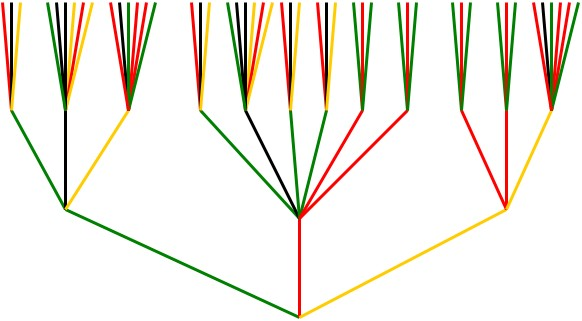
\includegraphics[width=5in]{V-vargenBB.jpg} 
   \caption{\small The construction tree corresponding to cell development  as in Figure~\ref{V-vargenA} for an initial red cell.}
   \label{V-vargenBB}
\end{figure}

In the example corresponding to   Figure~\ref{V-vargenA} each node of the tree will correspond to an IFS $ SG(2) $ or $ SG(3) $, the edges coming out of the node will correspond to $ f_1,f_2,f_3$ or $ g_1,\dots, g_6 $ respectively as in Figure~\ref{SG} when reading the tree from left to right, and the branch colour have the same role as in Figure~\ref{V-vargenA}.  In this case the labels at a node  are determined by the number of edges coming out of the node, 3 for $ SG(2) $ and   6 for $ SG(3) $.

Note that at each level the subtree rooted at the upper end of each edge is the same for all edges of the same colour.  This is essentially the $ V $-variable feature of the fractals considered here.

We also note again that the colours are important in the construction process, but each prefractal is obtained from the corresponding tree without the colours playing a role.   

%%%%%%%%%%%%%%%%%%%%%%%%%%%%%%%%%%%%%%
\subsection{Comparison with Other Notions}
In order to compare with other notions in the literature we note the following.  

\begin{enumerate}
\item \emph{Homogeneous fractals}: These correspond to trees where $ V=1 $, there is only one colour or type and so it no longer plays a role, and the subtrees rooted at each fixed level are the same.  In particular, for each $ k $ there is either 3-fold branching or 6-fold branching at all nodes at level $ k $. 

\item \emph{Recursive fractals}:  These correspond to trees where there are no colours  or types, and the subtree rooted at any node can be either 3-fold or 6-fold branching, without any constraint as a result of what happens at other nodes at the same or different levels.

\item \emph{Recursive graph directed fractals}:  Here we recall the construction in pages 8--12 of the book of Olsen.  

One begins with a directed multigraph $ (\mathcal{V} , E ) $ where $ \mathcal{V} $ is the set of vertices and  $ E$ is the set of edges. Let $ E_u $ be the set of edges with initial vertex $ u $.
There are compact metric spaces $ X_u $ for each   
$ u \in \mathcal{V} $. In Figure~\ref{V-vargenA} the spaces $ X_u $ will correspond to 4 disjoint compact subsets of $ \mathbb{R}^2 $ containing the 4 prefractals constructed at each level of approximation.  
For each  $ u \in \mathcal{V} $   there is   a collection of contractive maps 
\[
\mathcal{S}_u = \{ S_e  \mid   e\in E_u ,\ S_e : X_{v} \to X_u \text{ where $v $ is the terminal vertex of $ e $} \}.
\]

Using these ingredients     one constructs the class of what we call the recursive graph directed fractals ---  the class of fractals   which  are realisations of random self-similar sets in the sense of Olsen.   Each such fractal can be made to correspond  to a (complicated) labelled construction tree.

The essential difference between recursive graph directed fractals and $ V $-variable fractals is that in the latter case there are at most $ V $ distinct subtrees rooted at each level.  The recursive graph directed fractals impose no such restriction, and in fact generalise    the notion of  a recursive  fractal in (2) above.
\end{enumerate} 

It is the ``$ V $ distinct subtrees rooted at each level'' property of   $ V $-variable fractals which allows one to run a forward process that approximates the class of all possible $ V $-variable fractals.  We discuss this more carefully later.
  There is a forward process for  approximating  a standard graph directed fractals, analogous to that for approximating a standard IFS fractal.  But there is not a corresponding forward process which approximates the class of recursive graph directed fractals.




%%%%%%%%%%%%%%%%%%%%%%%%%%%%%%%%%%%%%
\subsection{Probabilistic Version}  *** Incomplete***
Now let $ P $ be  a probability distribution   on   $ \mathfrak{F} $.   If $ \mathfrak{F} $ is obtained from a family of IFSs as in Section~\ref{mcw} then 




Suppose the $ V $ transformation rules (IFSs) at each generation are selected in an iid manner according to $ P $,   and  independently of the rules selected  at any other generation. This induces a probability distribution  on the construction process and hence a probability distribution $ P_V $ on the set of generated fractals.   

 $ P_1 $ is the usual probability distribution on homogeneous random fractals.  $ P_V \to  P_\infty $ in the weak sense as $ V \to \infty $, where $ P_\infty $ is the standard distribution for random recursive fractals.  

%%%%%%%%%%%%%%%%%%%%%%%%%%%%%%%%
%%%%%%%%%%%%%%%%%%%%%%%%%%%%%%%%
%%%%%%%%%%%%%%%%%%%%%%%%%%%%%%%%
%%%%%%%%%%%%%%%%%%%%%%%%%%%%%%%%
\section{\textbf{11/2/10: Summary for $ V $-variable Fractals}} 

 In the following   fix a positive integer $ V $ and a family $ \boldsymbol{F} $ of IFSs.

\begin{definition}  An \emph{IFS tree $ T $} is  a    tree with the following properties: 
\begin{enumerate}
\item there is a single, level 0, root node $ \emptyset $;
\item the \emph{branching number} $ n^{\boldsymbol{i}} \geq 2 $   at   each node $ \boldsymbol{i}  $ is finite and $ \geq 2 $;
\item the  edges with  initial node $ \boldsymbol{i} $ are numbered (``left to right'') from $ 1,\dots, n^{\boldsymbol{i}} $;      we   write $ \boldsymbol{i} = i_1\dots i_{k }$ in the usual manner where $| \boldsymbol{i} | := k \geq 1$ is the \emph{level} of $ \boldsymbol{i}$;
\item there is an \emph{IFS} $ F^{ \boldsymbol{i} } \in \boldsymbol{F} $ associated with each node $ \boldsymbol{i} $,  $ n^ {\boldsymbol{i}} = |  F^{ \boldsymbol{i} } |  $ (the cardinality of $  F^{ \boldsymbol{i} }$), and the $k $th edge with initial node $ \boldsymbol{i} $ is associated with the $ k  $th function in the IFS $ F^{ \boldsymbol{i}}$.
\end{enumerate} 
The   unique compact set $ K = K(T)$ associated with $ T $ in the usual manner is called a \emph{$ V $-variable fractal}.
\end{definition} 

\medskip For   approximations to an IFS tree and the associated  fractal, see  Figure *** but  \emph{ignore} the ``environments'' and the symbols for the ``types'' $ \{12,3,4\}$.  In this example $ \boldsymbol{F} = \{F(2), F(3)\} $  contains the IFSs generating $ SG(2) $ and $ SG(3) $ respectively, and the IFS at each node is  determined by the branching number at the node.
Looking at the top tree in the Figure, we see that at the base node the IFS is $ F(3) $, and at the level one nodes, from left to right, the IFSs are $F(2), F(2), F(2), F(3), F(3), F(2) $.

The fractal is obtained by first applying $ F(3) $ and it corresponds to $ SG(3) $ at   level one.  At   level 2, reading anticlockwise from the bottom left corner, the fractal is obtained by applying $  F(2), F(2), F(2), F(3), F(3), F(2) $, and corresponds to $SG(2), SG(2), SG(2), SG(3), SG(3), SG(2) $.




\begin{definition} \label{dfVt}
Suppose $ V $ is a positive integer.   A  \emph{$ V $-variable IFS tree} is an IFS tree $ T $ with a \emph{type} $ \tau  ^{ \boldsymbol{i} } \in \{1,\dots, V \} $ associated to each node $ \boldsymbol{i} $, such that  if two nodes at the \emph{same} level $ k $  have the same type then:
\begin{enumerate}
\item   both nodes have the same branching number and   associated IFS, i.e.
\[ 
 |\boldsymbol{i} | = | \boldsymbol{j} | \ \&\ \tau ^{\boldsymbol{i}}= \tau ^{\boldsymbol{j} }
 \    \Longrightarrow \ n^ { \boldsymbol{i} } = n^ { \boldsymbol{j} }  \ \& \ F^ { \boldsymbol{i} } = F^ { \boldsymbol{j} } ;
     \]
    
    \item   comparable successor nodes   have the same type as each other, i.e.
    \[
 |\boldsymbol{i} | = | \boldsymbol{j} | \ \&\ \tau ^{\boldsymbol{i}}= \tau ^{\boldsymbol{j} }
\ \&\ 1 \leq p \leq  n^ { \boldsymbol{i} }  \  \Longrightarrow \ 
\tau ^{ \boldsymbol{i}  p } =   \tau ^{ \boldsymbol{j}  p } .
\]
    \end{enumerate} 
\end{definition}     
    
\begin{remark} \mbox{}

    \begin{enumerate}
 \item A  1-variable IFS tree  is essentially the same as an IFS tree  which generate a scale irregular, i.e.\ homogeneous, fractal.
    \item   A $ V $-variable IFS tree  has at most $  V $ distinct IFSs associated to the nodes at each fixed level.
    \item More strongly, if two nodes at the \emph{same} level  of  a $ V $-variable IFS tree have the same type then the subtrees rooted at these two nodes are identical, i.e.\
    \[
 | \boldsymbol{i} | = | \boldsymbol{j}  |
  \ \&\ \tau ^{\boldsymbol{i}}= \tau ^{\boldsymbol{j} }
  \  \Longrightarrow\  \sigma _{ \boldsymbol{i} } T = \sigma _ { \boldsymbol{j} } T .
 \]
In particular there are at most $ V $ distinct subtrees rooted at the \emph{same} level.
 \end{enumerate} 
\hfill $\square$  \end{remark}  

The following is used in the construction and analysis of $ V $-variable fractals.

\begin{definition} \label{dfenv}  An \emph{environment} $ \mathcal{E}$ assigns to each type $v \in \{1,\dots, V \} $ an  IFS $ F= F_v \in \boldsymbol{F} $ and a sequence of types $( \tau_{v1}, \dots, \tau_{vn})$, where $ n = |F_v| $.  We write 
\[
%\mathcal{E} = (E_1,\dots, E_V),\quad   E_v = (F(v),  \tau_{v1}, \dots,  \tau_{v |F(v)|  }). 
\mathcal{E} = (E^{\mathcal{E}}_1,\dots, E^{\mathcal{E}}_V),\quad   E^{\mathcal{E}}_v 
       = (F^{\mathcal{E}}_v,  \tau^{\mathcal{E}}_{v1}, \dots,  \tau^{\mathcal{E}}_{v n }). 
\]
\end{definition} 
 
 
\begin{remark}[Construction of $ V $-variable IFS trees]  
 $ V $-variable IFS trees are constructed recursively  as follows:
\begin{enumerate}

\item \emph{Stage 0}:  Assign a type $ \tau^\emptyset $ to the root node $ \emptyset $.
 
\item Assume that by the completion of stages $ 0$  to $  n-1$: 
\begin{enumerate}
\item the tree and all nodes $ \boldsymbol{i} $ with  $ | \boldsymbol{i} | \leq n-1 $ have been constructed,
\item a type $ \tau ^ { \boldsymbol{i} } $ has been assigned if  $ | \boldsymbol{i} | \leq n-1 $, 
\item an IFS $F ^ { \boldsymbol{i} } $ has been assigned if  $ | \boldsymbol{i} | \leq n-2 $, 
\item  the two properties in Definition~\ref{dfVt}  hold if  $ | \boldsymbol{i} | \leq n-2 $.
\end{enumerate}  

\item   \emph{Stage n}:  Choose an environment $ \mathcal{E} $.  We follow the notation of Definition~\ref{dfenv}  and use $ \mathcal{E}  $ in the obvious way to assign a type to the level $ n-1 $ nodes, to construct the level $ n $ nodes, and to assign a type to every level $ n $ node.  
 
 More precisely, for each node $ \boldsymbol{i} $ with  $ | \boldsymbol{i} | = n -1 $:
\begin{enumerate}
\item if $ v =\tau ^ {\boldsymbol{i} }  $ is the type already assigned to $ \boldsymbol{i} $, then   $ F^{\boldsymbol{i}} := F^{\mathcal{E} }_v$   is the IFS assigned to $ \boldsymbol{i} $, 
\item the branching number at $ \boldsymbol{i} $ is $ |F^{\boldsymbol{i}}| $,
\item for $ 1\leq u \leq |F^{\boldsymbol{i}}| $ the type $\tau ^{\boldsymbol{i} u } := \tau^{\mathcal{E}}_{vu} $ is the type assigned to the  node $ \boldsymbol{i} u $ .
\end{enumerate} 
\end{enumerate} 

It follows by an easy induction that the properties in  Definition~\ref{dfVt} hold at all nodes.
\hfill $\square$  \end{remark} 

\begin{definition} The environment $ \mathcal{E} $ in Definition~\ref{dfenv}  is a \emph{neck}  if all $ \tau _{uv} ^{\mathcal{E} } $ are equal.

A \emph{neck} occurs at level $ n $ in the construction of a $ V $-variable IFS tree if the environment $ \mathcal{E} $ applied at stage $ n $ is a neck environment.
\end{definition} 

If a neck occurs at level $ n $  then the type assigned to every node at that level is the same. It follows that the IFS assigned to every node at level $ n $ will be the same, and moreover all (infinite) subtrees rooted at level $ n $ will be the same. But the subtrees themselves are only constructed at later stages, and even  the common  value of the IFS at each level $ n $ node is not determined until stage $ n+1 $.  

There is no restriction on the IFSs occurring in the environment $ \mathcal{E} $; these IFSs are applied at level $ n-1 $.  


\begin{definition} Fix a probability distribution $ P $ on $ \boldsymbol{F} $.  This induces a probability distribution $ P_V $ on the set of environments $ \mathcal{E} $ by first choosing the IFSs $ F^{\mathcal{E} } _v $ for $ v \in \{1,\dots,V\} $ in an iid manner according to $ P $.   The types $ \tau ^{\mathcal{E}} _{uv} $ for the same range of $ v $ and for $ 1 \leq u \leq | F^{\mathcal{E} } _v | $ are chosen in an iid manner according to the uniform distribution on $ \{1,\dots, V \} $ and independently of the  $ F^{\mathcal{E} } _v$, except that the cardinality  of  the set of such types depends on the cardinality of the chosen IFSs.

The probability distribution on the set of $ V $-variable IFS trees is obtained by choosing $ \tau ^\emptyset $ according to the uniform distribution and independently choosing the environments at each sage in an iid manner according to $ P_V $. This probability distribution on IFS trees induces a probability distribution of $ V $-variable fractals.  Both the distributions on trees and on fractals are also denoted by $ P_V $.
\end{definition}

Note that although the distribution $ P_V $ on environments is a product measure, this is very far from the case for the corresponding distribution on trees and on fractals.  There is a very high degree of dependency between the types (and hence the IFSs) assigned to two different nodes at the same level. 

Note also that necks will occur infinitely often



%%%%%%%%%%%%%%%%%%%%%%%%%%%%%%%%
%%%%%%%%%%%%%%%%%%%%%%%%%%%%%%%%
%%%%%%%%%%%%%%%%%%%%%%%%%%%%%%%%
%%%%%%%%%%%%%%%%%%%%%%%%%%%%%%%%
\section{\textbf{8/4/09: Analysis on Fractals via Flat Chains}} 

Could one use the flat chain setting (end of my 81 paper), together  with boundary operators as in Peres and Lyons book, "PROBABILITY ON TREES  AND NETWORKS'', section 2.4, to develop analysis on pcf and other fractals?


%%%%%%%%%%%%%%%%%%%%%%%%%%%%%%%%
%%%%%%%%%%%%%%%%%%%%%%%%%%%%%%%%
%%%%%%%%%%%%%%%%%%%%%%%%%%%%%%%%
%%%%%%%%%%%%%%%%%%%%%%%%%%%%%%%%
\section{\textbf{7/11/09: Evolving Galaxies}} 

Could one use the ideas of optimal transport in Ch 8 of Villani, Yopics in Optimal Transportation,  to get a fractal limiting distribution?

%%%%%%%%%%%%%%%%%%%%%%%%%%%%%%%%
%%%%%%%%%%%%%%%%%%%%%%%%%%%%%%%%
%%%%%%%%%%%%%%%%%%%%%%%%%%%%%%%%
%%%%%%%%%%%%%%%%%%%%%%%%%%%%%%%%
%%%%%%%%%%%%%%%%%%%%%%%%%%%%%%%%%%%%
\begin{thebibliography}{9} 

   \bib{BHS}{article}{
    author={Barnsley, M. F.},
    author={Hutchinson, John E.},
    author={Stenflo, {\"O}rjan},
    title={V-variable Fractals: Dimension results},
   note={submitted for publication},   
   date={2009},   
}


\bib{Sce1}{thesis}{
   author={Scealy, Bob},
   title={V-variable fractals and interpolation},
  note={draft Version, 7 September}, 
  date={2007}
     }

\bib{Sce2}{thesis}{
   author={Scealy, Bob},
   title={V-variable fractals and interpolation},
%  note={Preliminary Version, 7 September 2007}, 
  date={2008}
     }

\end{thebibliography} 
\end{document} 






\begin{figure}[htbp] %  figure placement: here, top, bottom, or page
   \centering
   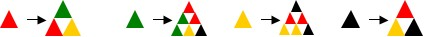
\includegraphics[width=5in]{V-vargen1T.jpg} \\ \mbox{} \\
   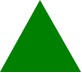
\includegraphics[width=1in]{V-vargen0.jpg} \hspace{5cm}
   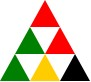
\includegraphics[width=1in]{V-vargen1.jpg} 
   \caption{Initial cell of type green.  The 4 transformation rules at time 1 (only the second is relevant).  The resulting organism at time 1.}
   \label{V-vargen1}
\end{figure}




\begin{figure}[htbp] %  figure placement: here, top, bottom, or page
   \centering
   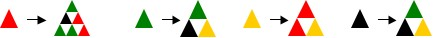
\includegraphics[width=5in]{V-vargen2T.jpg} \\ \mbox{} \\
   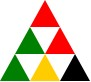
\includegraphics[width=1in]{V-vargen1.jpg}  \hspace{4cm}
    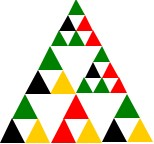
\includegraphics[width=1in]{V-vargen2.jpg} 
   \caption{The organism at time 1. The transformation rules at time 2. The resulting organism at time 2.}
   \label{V-vargen2}
\end{figure}
 










\begin{figure}[htbp] %  figure placement: here, top, bottom, or page
   \centering
   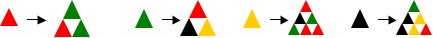
\includegraphics[width=5in]{V-vargen3T.jpg} \\ \mbox{} \\
   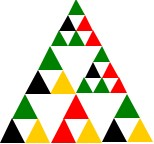
\includegraphics[width=2.2in, height=2in]{V-vargen2.jpg}  \hspace{2cm}
    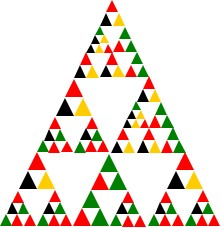
\includegraphics[width=2.2in, height=2in]{V-vargen3.jpg} 
   \caption{the organism at time 2. The transformation rules at time 3.  The resulting organism at time 3.}
   \label{V-vargen3}
\end{figure}
 
%%%%%%%%%%%%%%%%%%%%%%%%%%%%%%%%%%%%%%%%%%%


%%%%%%%%%%%%%%%%%%%%%%%%%%%%%%%%%%%%%%%%%
%%%%%%%%%%%%%%%%%%%%%%%%%%%%%%%%%%%%%%%%%
\newpage \subsection{Backward Process}   See Figure~\ref{g3sg}.



\begin{figure}[htbp] %  figure placement: here, top, bottom, or page
   \centering
   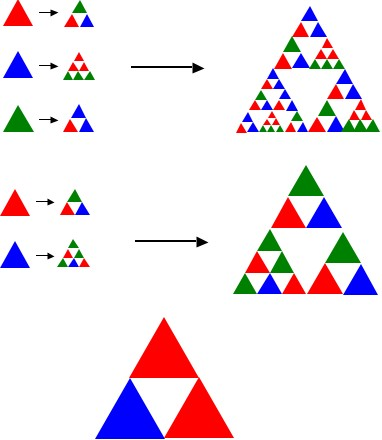
\includegraphics[width=3.5in]{V-cat.jpg} 
   \caption{Level 1, 2 and 3 prefractals in the generation process  for a 3-variable Sierpinski Gasket.
   On the left of the large arrows are indicated the IFSs used to transform the red, blue and green cells at the previous level.  The partitions of the new cells into red, blue and green are also indicated.}
   \label{g3sg}
\end{figure}

\begin{figure}[htbp] %  figure placement: here, top, bottom, or page
   \centering
   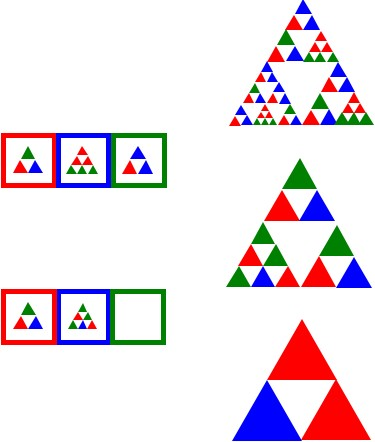
\includegraphics[width=3.5in]{V-cat2.jpg} 
   \caption{Box representation of the same example.  The red, blue and green boxes show the IFSs used to transform the red, blue and green cells at the previous level.  The partitions of the new cells into red, blue and green are also indicated.}
   \label{g3sg2}
\end{figure}


Given data consists of a family $ \mathcal{F} $ of IFS's $ \{ F^ \lambda = (\psi^  \lambda _1,\dots, \psi^ \lambda _{M_\lambda });   \lambda \in \Lambda  \}$,    a natural number  $ V \geq 1 $ and a probability distribution $ P $ on $ \Lambda $.

For the example in Figure~\ref{g3sg}, $ \mathcal{F} $ contains the two IFSs
$F^2= (\psi^2_1,\psi^2_2,\psi^2_3)  $ and $F^3= (\psi^3_1,\dots,\psi^3_6)  $ generating $ SG(2) $ and $ SG(3) $ respectively.
The corresponding probability distribution is given by  $ P(2) = p $ and $ P(3) = q $.

\medskip Each realisation%
\footnote{Not just a.e.\ realisation.}
$ \omega $ of the generation process  produces 
 a sequence of level $ n $ prefractals $ G^n = G^n(\omega) $ whose limit $ G = G(\omega) $ is a $ V  $-variable fractal.
 The probability $ P $ is not required for this.

The probability distribution  $ P $  gives a natural probability distribution on the generation process such that $ \omega \mapsto G(\omega) $ is a random $ V $-variable fractal with a natural probability distribution.


\medskip
It is helpful to assume each $ F^ \lambda $ is pcf with a common base set  $ V^{(0)} $.  In Figure~\ref{g3sg}, $ V^{(0)} $ is interpreted as the set of vertices of the standard equilateral triangle in~$ \mathbb{R}^2 $.  

Alternatively, assume that there is a compact subset $ T $ independent of $ \lambda $ such that $ F^ \lambda (T) \subset T $ for each $ \lambda $.  In Figure~\ref{g3sg}, $ T $ is the closed convex hull of the standard equilateral triangle in~$ \mathbb{R}^2 $. 

\medskip
The case $ V=1 $  corresponds to the homogeneous random fractal case.
The case $ V $ large approximates the random recursive case.  

%%%%%%%%%%%%%%%%%%%%%%%%%%
\subsubsection{Summary}  (The process can be applied with or without using the probability distribution $ P $.  The probabilistic aspects of the construction are in parentheses.)

In the first step an IFS is chosen (via $ P $), a level 1 prefractal is obtained by applying this IFS to the level 0 prefractal common to all the IFSs, and the resulting 1-cells are partitioned   into   $ V $ equivalence classes (each 1-cell independently according to the uniform distribution on $\{ 1,\dots, V \}$).

After  step $ n $ for $ n\geq 1$, one has obtained a level $ n $ prefractal together with a partition of its $ n $-cells  into $ V $ equivalence classes. 
In the subsequent step $ n + 1 $ one selects an IFS for each of these $ V $ equivalence classes of $ n $-cells (independently according to $ P $), applies this \emph{same} IFS to \emph{each} $ n $-cell in the equivalence class, and partitions the resulting $ n+1 $-cells into  $ V $ equivalence classes (independently for the $ n+1 $-cells corresponding to a fixed $ n$-cell) and in the \emph{``same''} way for the $ n+1 $-cell ``children'' of each $ n $-cell in the same equivalence class. 


%%%%%%%%%%%%%%%%%%%%%%%%%%%

\subsubsection{Details} 
\begin{enumerate}
\item The level 1 prefractal is obtained by applying $ F^\lambda $ to $  V^{(0)} $ or to $ T $, and then partitioning the resulting 1-cells into $ V $  possibly empty equivalence classes.  

(In the probabilistic case $ F^\lambda $ is chosen via $ P $.  The equivalence class  for each 1-cell is then chosen independently according to the uniform distribution.)


In Figure~\ref{g3sg}  see the bottom row, where the IFS $ F^2 $ is applied and equivalence classes of 1-cells are represented by   red, blue and green (the latter class is empty in the example).

\item The level 2 prefractal is obtained by applying an  $ F^\lambda $ to each 1-cell in the level 1 prefractal and partitioning the resulting 2-cells into $ V $  possibly empty equivalence classes.  The same IFS is applied to equivalent 1-cells and the same partition is then applied to the resulting 2-cells.

(In the probabilistic case the IFS for each equivalence class  is chosen independently via $ P $.  For a fixed 1-cell the equivalence class  for each resulting  2-cell is chosen independently  according to the uniform distribution.  The ``same'' partition is used for every 1-cell in the same equivalence class, but different equivalence classes are treated independently.)

In Figure~\ref{g3sg}  the non empty classes of 1-cells correspond to red and blue, the corresponding IFS and partitions are indicated on the left of the middle row of figures, and the resulting  level 2 prefractal with its partition of 2-cells is shown on the right.

\item  The level 3 prefractal is obtained by applying some  $ F^\lambda $ to each 2-cell in the level 2 prefractal and partitioning the resulting 3-cells into $ V $  possibly empty equivalence classes.  The same IFS is applied to equivalent 2-cells and the same partition is then applied to the resulting 3-cells.

(In the probabilistic case the IFS for each equivalence class  is chosen independently via $ P $.  For a fixed 2-cell the equivalence classes for each resulting  3-cell is chosen independently   according to the uniform distribution. The ``same'' partition is used for every 2-cell in the same equivalence class, but different equivalence classes are treated independently.)

In Figure~\ref{g3sg} the  equivalence classes of 1-cells again correspond to red, blue and green; the corresponding IFS and partitions are indicated on the left of the top row of figures, and the resulting  level 3 prefractal with its partition of 3-cells is shown on the right.
\end{enumerate} 
 

%%%%%%%%%%%%%%%%%%%%%%%%%%%%%%%%%%%%%%%%%
\subsection{Forward Process}  


